 \documentclass{beamer}

\usetheme{MagdeburgFIN}
\usefonttheme{structurebold}
\usepackage{graphicx}
\usepackage{float}
\usepackage{url}
\usepackage{pdfpages}
\usepackage[ngerman]{babel}
\usepackage[utf8]{inputenc}

\title{Scientific Team Project}
\subtitle{Thread Pool in GeckoDB/BOLSTER}
\author{Johann Wagner, Johannes Wünsche, Marten Wallewein-Eising, Robert Jenderise, Benedikt Zeilinger}
\date{\today}
\institute{Otto von Guericke University, Magdeburg}

%Topic, schedule, and team presentation & first results of literature research

\begin{document}

\begin{frame}[plain]
 \titlepage
\end{frame}



\section[Agenda]{}
	\begin{frame}
	\frametitle{Agenda}
	\tableofcontents
	\end{frame}

\section{Introduction}
	\begin{frame}
		\frametitle{Introduction}
		\begin{itemize}
			\item \emph{In computer programming, a thread pool is a software design pattern for achieving concurrency of execution in a computer program.}
			\item Pool of Threads
			\item Reduces overhead of creating new threads by reusing existing threads.
		\end{itemize}
	\end{frame}
	
	\begin{frame}
		\frametitle{Team Roles}
		\begin{figure}
			\centering
			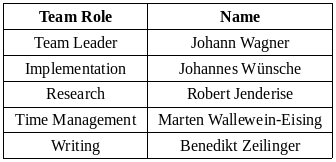
\includegraphics[width=0.7\linewidth]{img/TeamRoles}
			\caption{}
			\label{fig:teamroles}
		\end{figure}
	\end{frame}
	
	\begin{frame}
		\frametitle{Current Situation}
		\begin{itemize}
			\item Operations are spawning dozens of threads, which are not handled and managed..
			\item After some operations profilers dies.
		\end{itemize}
	\end{frame}

	\begin{frame}
		\frametitle{Desirable Situation}
		\begin{itemize}
			\item Reuse of Threads with thread pools.
			\item Limited amount of threads, which are handled correctly.
		\end{itemize}
	\end{frame}

\section{Planning}
\begin{frame}
\frametitle{Schedule}
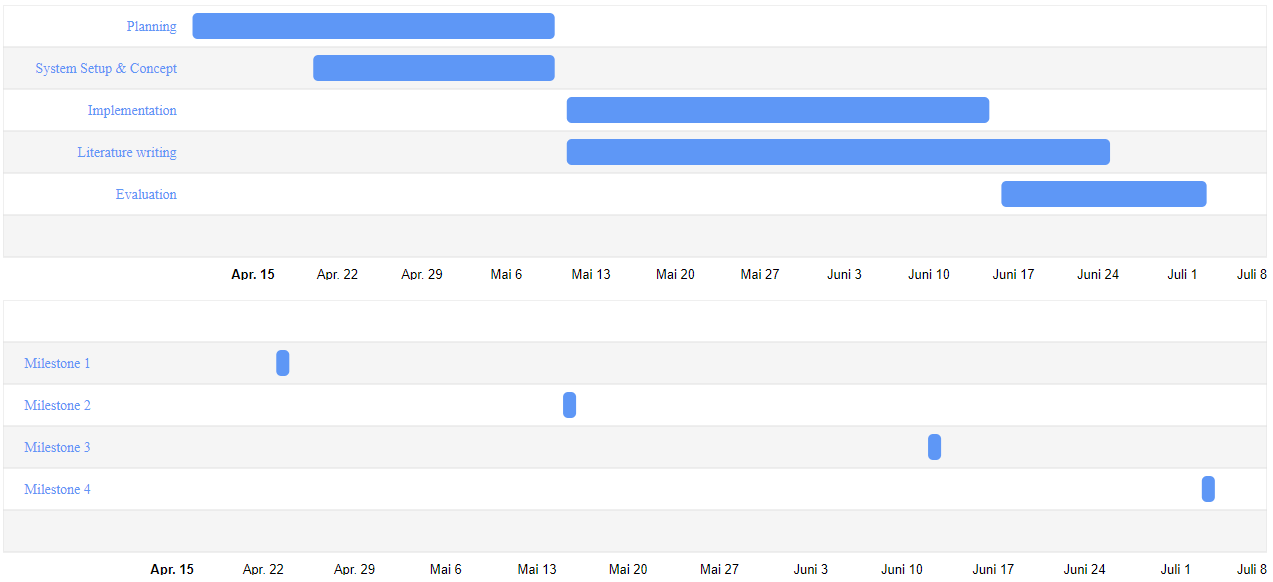
\includegraphics[width=1.0\textwidth]{img/schedule.png}
\end{frame}

\section{Literature Research}
    \begin{frame}
        \frametitle{Literature Research}
        \begin{itemize}
            \item Xu, Dongping, and Brett Bode. \emph{"Performance study and dynamic optimization design for thread pool systems".} Diss. United States. Department of Energy. Office of Science, 2004.
            \item Ling, Yibei, Tracy Mullen, and Xiaola Lin. \emph{Analysis of optimal thread pool size.} ACM SIGOPS Operating Systems Review 34.2 (2000): 42-55.
            \item Kang, DongHyun, et al. \emph{Prediction-based dynamic thread pool scheme for efficient resource usage.} Computer and Information Technology Workshops, 2008. CIT Workshops 2008. IEEE 8th International Conference on. IEEE, 2008.
        \end{itemize}
    \end{frame}

    \begin{frame}
        \frametitle{Thank you for your attention!}
    \end{frame}
\end{document}
